\documentclass[twoside]{book}

% Packages required by doxygen
\usepackage{fixltx2e}
\usepackage{calc}
\usepackage{doxygen}
\usepackage[export]{adjustbox} % also loads graphicx
\usepackage{graphicx}
\usepackage[utf8]{inputenc}
\usepackage{makeidx}
\usepackage{multicol}
\usepackage{multirow}
\PassOptionsToPackage{warn}{textcomp}
\usepackage{textcomp}
\usepackage[nointegrals]{wasysym}
\usepackage[table]{xcolor}

% Font selection
\usepackage[T1]{fontenc}
\usepackage[scaled=.90]{helvet}
\usepackage{courier}
\usepackage{amssymb}
\usepackage{sectsty}
\renewcommand{\familydefault}{\sfdefault}
\allsectionsfont{%
  \fontseries{bc}\selectfont%
  \color{darkgray}%
}
\renewcommand{\DoxyLabelFont}{%
  \fontseries{bc}\selectfont%
  \color{darkgray}%
}
\newcommand{\+}{\discretionary{\mbox{\scriptsize$\hookleftarrow$}}{}{}}

% Page & text layout
\usepackage{geometry}
\geometry{%
  a4paper,%
  top=2.5cm,%
  bottom=2.5cm,%
  left=2.5cm,%
  right=2.5cm%
}
\tolerance=750
\hfuzz=15pt
\hbadness=750
\setlength{\emergencystretch}{15pt}
\setlength{\parindent}{0cm}
\setlength{\parskip}{0.2cm}
\makeatletter
\renewcommand{\paragraph}{%
  \@startsection{paragraph}{4}{0ex}{-1.0ex}{1.0ex}{%
    \normalfont\normalsize\bfseries\SS@parafont%
  }%
}
\renewcommand{\subparagraph}{%
  \@startsection{subparagraph}{5}{0ex}{-1.0ex}{1.0ex}{%
    \normalfont\normalsize\bfseries\SS@subparafont%
  }%
}
\makeatother

% Headers & footers
\usepackage{fancyhdr}
\pagestyle{fancyplain}
\fancyhead[LE]{\fancyplain{}{\bfseries\thepage}}
\fancyhead[CE]{\fancyplain{}{}}
\fancyhead[RE]{\fancyplain{}{\bfseries\leftmark}}
\fancyhead[LO]{\fancyplain{}{\bfseries\rightmark}}
\fancyhead[CO]{\fancyplain{}{}}
\fancyhead[RO]{\fancyplain{}{\bfseries\thepage}}
\fancyfoot[LE]{\fancyplain{}{}}
\fancyfoot[CE]{\fancyplain{}{}}
\fancyfoot[RE]{\fancyplain{}{\bfseries\scriptsize Generated on Mon Mar 30 2015 17\+:05\+:52 for Z\+S\+T Klient by Doxygen }}
\fancyfoot[LO]{\fancyplain{}{\bfseries\scriptsize Generated on Mon Mar 30 2015 17\+:05\+:52 for Z\+S\+T Klient by Doxygen }}
\fancyfoot[CO]{\fancyplain{}{}}
\fancyfoot[RO]{\fancyplain{}{}}
\renewcommand{\footrulewidth}{0.4pt}
\renewcommand{\chaptermark}[1]{%
  \markboth{#1}{}%
}
\renewcommand{\sectionmark}[1]{%
  \markright{\thesection\ #1}%
}

% Indices & bibliography
\usepackage{natbib}
\usepackage[titles]{tocloft}
\setcounter{tocdepth}{3}
\setcounter{secnumdepth}{5}
\makeindex

% Hyperlinks (required, but should be loaded last)
\usepackage{ifpdf}
\ifpdf
  \usepackage[pdftex,pagebackref=true]{hyperref}
\else
  \usepackage[ps2pdf,pagebackref=true]{hyperref}
\fi
\hypersetup{%
  colorlinks=true,%
  linkcolor=blue,%
  citecolor=blue,%
  unicode%
}

% Custom commands
\newcommand{\clearemptydoublepage}{%
  \newpage{\pagestyle{empty}\cleardoublepage}%
}


%===== C O N T E N T S =====

\begin{document}

% Titlepage & ToC
\hypersetup{pageanchor=false,
             bookmarks=true,
             bookmarksnumbered=true,
             pdfencoding=unicode
            }
\pagenumbering{roman}
\begin{titlepage}
\vspace*{7cm}
\begin{center}%
{\Large Z\+S\+T Klient \\[1ex]\large 1.\+0 }\\
\vspace*{1cm}
{\large Generated by Doxygen 1.8.9.1}\\
\vspace*{0.5cm}
{\small Mon Mar 30 2015 17:05:52}\\
\end{center}
\end{titlepage}
\clearemptydoublepage
\tableofcontents
\clearemptydoublepage
\pagenumbering{arabic}
\hypersetup{pageanchor=true}

%--- Begin generated contents ---
\chapter{Namespace Index}
\section{Pakiety}
Oto lista pakietów wraz z krótkim opisem (o ile jest dostępny)\+:\begin{DoxyCompactList}
\item\contentsline{section}{\hyperlink{namespace_z_s_t}{Z\+S\+T} }{\pageref{namespace_z_s_t}}{}
\item\contentsline{section}{\hyperlink{namespace_z_s_t_1_1_properties}{Z\+S\+T.\+Properties} }{\pageref{namespace_z_s_t_1_1_properties}}{}
\end{DoxyCompactList}

\chapter{Hierarchical Index}
\section{Hierarchia klas}
Ta lista dziedziczenia posortowana jest z grubsza, choć nie całkowicie, alfabetycznie\+:\begin{DoxyCompactList}
\item Event\+Args\begin{DoxyCompactList}
\item \contentsline{section}{Z\+S\+T.\+Log\+Args}{\pageref{class_z_s_t_1_1_log_args}}{}
\item \contentsline{section}{Z\+S\+T.\+New\+Log\+Args}{\pageref{class_z_s_t_1_1_new_log_args}}{}
\end{DoxyCompactList}
\item Form\begin{DoxyCompactList}
\item \contentsline{section}{Z\+S\+T.\+Form1}{\pageref{class_z_s_t_1_1_form1}}{}
\end{DoxyCompactList}
\item \contentsline{section}{Z\+S\+T.\+Log}{\pageref{class_z_s_t_1_1_log}}{}
\item \contentsline{section}{Z\+S\+T.\+Log\+Agent}{\pageref{class_z_s_t_1_1_log_agent}}{}
\item \contentsline{section}{Z\+S\+T.\+Log\+Viewer}{\pageref{class_z_s_t_1_1_log_viewer}}{}
\item \contentsline{section}{Z\+S\+T.\+Server}{\pageref{class_z_s_t_1_1_server}}{}
\end{DoxyCompactList}

\chapter{Class Index}
\section{Lista klas}
Tutaj znajdują się klasy, struktury, unie i interfejsy wraz z ich krótkimi opisami\+:\begin{DoxyCompactList}
\item\contentsline{section}{\hyperlink{class_z_s_t_1_1_form1}{Z\+S\+T.\+Form1} \\*Klasa reprezentująca okienko aplikacji }{\pageref{class_z_s_t_1_1_form1}}{}
\item\contentsline{section}{\hyperlink{class_z_s_t_1_1_log}{Z\+S\+T.\+Log} \\*Klasa reprezentująca pojedyńczy log (zapis w dzienniku zdarzen) }{\pageref{class_z_s_t_1_1_log}}{}
\item\contentsline{section}{\hyperlink{class_z_s_t_1_1_log_agent}{Z\+S\+T.\+Log\+Agent} \\*Klasa pozwalająca na zdalny zapis logów }{\pageref{class_z_s_t_1_1_log_agent}}{}
\item\contentsline{section}{\hyperlink{class_z_s_t_1_1_log_args}{Z\+S\+T.\+Log\+Args} \\*Klasa argumentów wysyłanego zdarzenia (przyjścia nowego logu z sieci) }{\pageref{class_z_s_t_1_1_log_args}}{}
\item\contentsline{section}{\hyperlink{class_z_s_t_1_1_log_viewer}{Z\+S\+T.\+Log\+Viewer} \\*Klasa reprezentująca wyświetlanie logów }{\pageref{class_z_s_t_1_1_log_viewer}}{}
\item\contentsline{section}{\hyperlink{class_z_s_t_1_1_server}{Z\+S\+T.\+Server} \\*Klasa serwera }{\pageref{class_z_s_t_1_1_server}}{}
\end{DoxyCompactList}

\chapter{File Index}
\section{Lista plików}
Tutaj znajduje się lista wszystkich plików z ich krótkimi opisami\+:\begin{DoxyCompactList}
\item\contentsline{section}{Z\+S\+T/\hyperlink{_form1_8cs}{Form1.\+cs} }{\pageref{_form1_8cs}}{}
\item\contentsline{section}{Z\+S\+T/\hyperlink{_form1_8_designer_8cs}{Form1.\+Designer.\+cs} }{\pageref{_form1_8_designer_8cs}}{}
\item\contentsline{section}{Z\+S\+T/\hyperlink{_log_8cs}{Log.\+cs} }{\pageref{_log_8cs}}{}
\item\contentsline{section}{Z\+S\+T/\hyperlink{_log_agent_8cs}{Log\+Agent.\+cs} }{\pageref{_log_agent_8cs}}{}
\item\contentsline{section}{Z\+S\+T/\hyperlink{_log_args_8cs}{Log\+Args.\+cs} }{\pageref{_log_args_8cs}}{}
\item\contentsline{section}{Z\+S\+T/\hyperlink{_log_viewer_8cs}{Log\+Viewer.\+cs} }{\pageref{_log_viewer_8cs}}{}
\item\contentsline{section}{Z\+S\+T/\hyperlink{_new_log_args_8cs}{New\+Log\+Args.\+cs} }{\pageref{_new_log_args_8cs}}{}
\item\contentsline{section}{Z\+S\+T/\hyperlink{_program_8cs}{Program.\+cs} }{\pageref{_program_8cs}}{}
\item\contentsline{section}{Z\+S\+T/\hyperlink{_server_8cs}{Server.\+cs} }{\pageref{_server_8cs}}{}
\item\contentsline{section}{Z\+S\+T/obj/\+Debug/\hyperlink{_temporary_generated_file__036_c0_b5_b-1481-4323-8_d20-8_f5_a_d_c_b23_d92_8cs}{Temporary\+Generated\+File\+\_\+036\+C0\+B5\+B-\/1481-\/4323-\/8\+D20-\/8\+F5\+A\+D\+C\+B23\+D92.\+cs} }{\pageref{_temporary_generated_file__036_c0_b5_b-1481-4323-8_d20-8_f5_a_d_c_b23_d92_8cs}}{}
\item\contentsline{section}{Z\+S\+T/obj/\+Debug/\hyperlink{_temporary_generated_file__5937a670-0e60-4077-877b-f7221da3dda1_8cs}{Temporary\+Generated\+File\+\_\+5937a670-\/0e60-\/4077-\/877b-\/f7221da3dda1.\+cs} }{\pageref{_temporary_generated_file__5937a670-0e60-4077-877b-f7221da3dda1_8cs}}{}
\item\contentsline{section}{Z\+S\+T/obj/\+Debug/\hyperlink{_temporary_generated_file___e7_a71_f73-0_f8_d-4_b9_b-_b56_e-8_e70_b10_b_c5_d3_8cs}{Temporary\+Generated\+File\+\_\+\+E7\+A71\+F73-\/0\+F8\+D-\/4\+B9\+B-\/\+B56\+E-\/8\+E70\+B10\+B\+C5\+D3.\+cs} }{\pageref{_temporary_generated_file___e7_a71_f73-0_f8_d-4_b9_b-_b56_e-8_e70_b10_b_c5_d3_8cs}}{}
\item\contentsline{section}{Z\+S\+T/\+Properties/\hyperlink{_assembly_info_8cs}{Assembly\+Info.\+cs} }{\pageref{_assembly_info_8cs}}{}
\item\contentsline{section}{Z\+S\+T/\+Properties/\hyperlink{_resources_8_designer_8cs}{Resources.\+Designer.\+cs} }{\pageref{_resources_8_designer_8cs}}{}
\item\contentsline{section}{Z\+S\+T/\+Properties/\hyperlink{_settings_8_designer_8cs}{Settings.\+Designer.\+cs} }{\pageref{_settings_8_designer_8cs}}{}
\end{DoxyCompactList}

\chapter{Namespace Documentation}
\hypertarget{namespace_windows_forms_application3}{}\section{Package Windows\+Forms\+Application3}
\label{namespace_windows_forms_application3}\index{Windows\+Forms\+Application3@{Windows\+Forms\+Application3}}
\subsection*{Namespaces}
\begin{DoxyCompactItemize}
\item 
package \hyperlink{namespace_windows_forms_application3_1_1_properties}{Properties}
\end{DoxyCompactItemize}
\subsection*{Classes}
\begin{DoxyCompactItemize}
\item 
class \hyperlink{class_windows_forms_application3_1_1_client}{Client}
\begin{DoxyCompactList}\small\item\em Klasa klienta \end{DoxyCompactList}\item 
class \hyperlink{class_windows_forms_application3_1_1_form1}{Form1}
\begin{DoxyCompactList}\small\item\em Klasa reprezentująca okno aplikacji \end{DoxyCompactList}\item 
class {\bfseries Program}
\end{DoxyCompactItemize}

\hypertarget{namespace_windows_forms_application3_1_1_properties}{}\section{Pakiet Windows\+Forms\+Application3.\+Properties}
\label{namespace_windows_forms_application3_1_1_properties}\index{Windows\+Forms\+Application3.\+Properties@{Windows\+Forms\+Application3.\+Properties}}
\subsection*{Komponenty}
\begin{DoxyCompactItemize}
\item 
class {\bfseries Resources}
\begin{DoxyCompactList}\small\item\em A strongly-\/typed resource class, for looking up localized strings, etc. \end{DoxyCompactList}\item 
class {\bfseries Settings}
\end{DoxyCompactItemize}

\chapter{Class Documentation}
\hypertarget{class_windows_forms_application3_1_1_client}{}\section{Windows\+Forms\+Application3.\+Client Class Reference}
\label{class_windows_forms_application3_1_1_client}\index{Windows\+Forms\+Application3.\+Client@{Windows\+Forms\+Application3.\+Client}}


Klasa klienta  


\subsection*{Public Member Functions}
\begin{DoxyCompactItemize}
\item 
\hyperlink{class_windows_forms_application3_1_1_client_a3ac0d5af309fb79e24fc58bd4d17a2b4}{Client} ()
\begin{DoxyCompactList}\small\item\em Konstruktor klasy klienta \end{DoxyCompactList}\item 
bool \hyperlink{class_windows_forms_application3_1_1_client_a9f9dfff8bba1fe20ca6d3da7cd706dd1}{connect} ()
\begin{DoxyCompactList}\small\item\em metoda łącząca klienta z serwerem \end{DoxyCompactList}\item 
void \hyperlink{class_windows_forms_application3_1_1_client_a136f39388b24a7e5bc498baefecd006d}{disconnect} (bool error=false)
\begin{DoxyCompactList}\small\item\em Rozłączenie klienta z serwerem \end{DoxyCompactList}\item 
void \hyperlink{class_windows_forms_application3_1_1_client_afcd6a12a5559cce41c20dba36bce0bc4}{send\+Message} (string msg)
\begin{DoxyCompactList}\small\item\em Wysyłanie wiadomości \end{DoxyCompactList}\end{DoxyCompactItemize}


\subsection{Detailed Description}
Klasa klienta 



\subsection{Constructor \& Destructor Documentation}
\hypertarget{class_windows_forms_application3_1_1_client_a3ac0d5af309fb79e24fc58bd4d17a2b4}{}\index{Windows\+Forms\+Application3\+::\+Client@{Windows\+Forms\+Application3\+::\+Client}!Client@{Client}}
\index{Client@{Client}!Windows\+Forms\+Application3\+::\+Client@{Windows\+Forms\+Application3\+::\+Client}}
\subsubsection[{Client}]{\setlength{\rightskip}{0pt plus 5cm}Windows\+Forms\+Application3.\+Client.\+Client (
\begin{DoxyParamCaption}
{}
\end{DoxyParamCaption}
)}\label{class_windows_forms_application3_1_1_client_a3ac0d5af309fb79e24fc58bd4d17a2b4}


Konstruktor klasy klienta 



\subsection{Member Function Documentation}
\hypertarget{class_windows_forms_application3_1_1_client_a9f9dfff8bba1fe20ca6d3da7cd706dd1}{}\index{Windows\+Forms\+Application3\+::\+Client@{Windows\+Forms\+Application3\+::\+Client}!connect@{connect}}
\index{connect@{connect}!Windows\+Forms\+Application3\+::\+Client@{Windows\+Forms\+Application3\+::\+Client}}
\subsubsection[{connect}]{\setlength{\rightskip}{0pt plus 5cm}bool Windows\+Forms\+Application3.\+Client.\+connect (
\begin{DoxyParamCaption}
{}
\end{DoxyParamCaption}
)}\label{class_windows_forms_application3_1_1_client_a9f9dfff8bba1fe20ca6d3da7cd706dd1}


metoda łącząca klienta z serwerem 

\begin{DoxyReturn}{Returns}
wynik operacji (powodzenia/niepowodzenie)
\end{DoxyReturn}
\hypertarget{class_windows_forms_application3_1_1_client_a136f39388b24a7e5bc498baefecd006d}{}\index{Windows\+Forms\+Application3\+::\+Client@{Windows\+Forms\+Application3\+::\+Client}!disconnect@{disconnect}}
\index{disconnect@{disconnect}!Windows\+Forms\+Application3\+::\+Client@{Windows\+Forms\+Application3\+::\+Client}}
\subsubsection[{disconnect}]{\setlength{\rightskip}{0pt plus 5cm}void Windows\+Forms\+Application3.\+Client.\+disconnect (
\begin{DoxyParamCaption}
\item[{bool}]{error = {\ttfamily false}}
\end{DoxyParamCaption}
)}\label{class_windows_forms_application3_1_1_client_a136f39388b24a7e5bc498baefecd006d}


Rozłączenie klienta z serwerem 


\begin{DoxyParams}{Parameters}
{\em error} & parametr określający czy rozłączenie wystąpiło z powodu błędu\\
\hline
\end{DoxyParams}
\hypertarget{class_windows_forms_application3_1_1_client_afcd6a12a5559cce41c20dba36bce0bc4}{}\index{Windows\+Forms\+Application3\+::\+Client@{Windows\+Forms\+Application3\+::\+Client}!send\+Message@{send\+Message}}
\index{send\+Message@{send\+Message}!Windows\+Forms\+Application3\+::\+Client@{Windows\+Forms\+Application3\+::\+Client}}
\subsubsection[{send\+Message}]{\setlength{\rightskip}{0pt plus 5cm}void Windows\+Forms\+Application3.\+Client.\+send\+Message (
\begin{DoxyParamCaption}
\item[{string}]{msg}
\end{DoxyParamCaption}
)}\label{class_windows_forms_application3_1_1_client_afcd6a12a5559cce41c20dba36bce0bc4}


Wysyłanie wiadomości 


\begin{DoxyParams}{Parameters}
{\em msg} & wiadomość do wysłania\\
\hline
\end{DoxyParams}


The documentation for this class was generated from the following file\+:\begin{DoxyCompactItemize}
\item 
Windows\+Forms\+Application3/\hyperlink{_client_8cs}{Client.\+cs}\end{DoxyCompactItemize}

\hypertarget{class_windows_forms_application3_1_1_form1}{}\section{Windows\+Forms\+Application3.\+Form1 Class Reference}
\label{class_windows_forms_application3_1_1_form1}\index{Windows\+Forms\+Application3.\+Form1@{Windows\+Forms\+Application3.\+Form1}}


Klasa reprezentująca okno aplikacji  


Inheritance diagram for Windows\+Forms\+Application3.\+Form1\+:\begin{figure}[H]
\begin{center}
\leavevmode
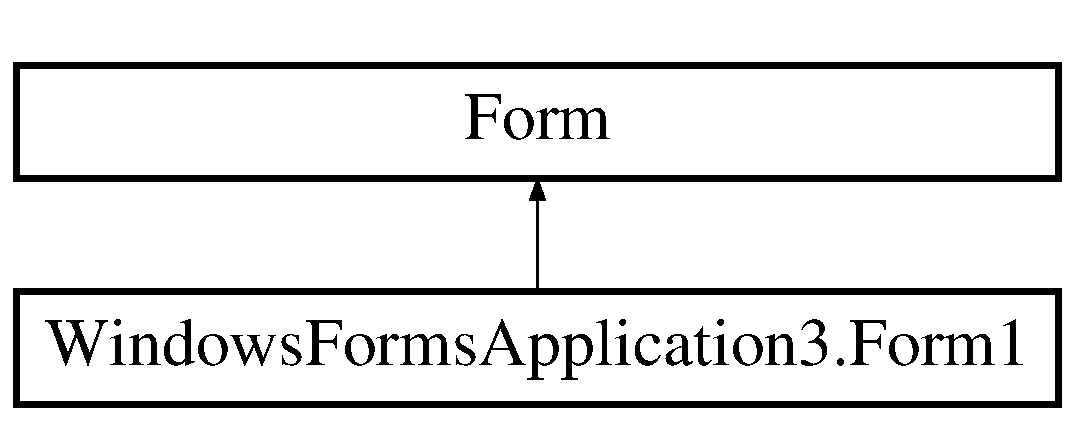
\includegraphics[height=2.000000cm]{class_windows_forms_application3_1_1_form1}
\end{center}
\end{figure}
\subsection*{Public Member Functions}
\begin{DoxyCompactItemize}
\item 
\hyperlink{class_windows_forms_application3_1_1_form1_a48366c981585157eeb906d8309bfa035}{Form1} ()
\begin{DoxyCompactList}\small\item\em Konstruktor klasy form \end{DoxyCompactList}\end{DoxyCompactItemize}
\subsection*{Protected Member Functions}
\begin{DoxyCompactItemize}
\item 
override void \hyperlink{class_windows_forms_application3_1_1_form1_a441acc637a89bc137cd3deb11d11ae43}{Dispose} (bool disposing)
\begin{DoxyCompactList}\small\item\em Clean up any resources being used. \end{DoxyCompactList}\end{DoxyCompactItemize}


\subsection{Detailed Description}
Klasa reprezentująca okno aplikacji 



\subsection{Constructor \& Destructor Documentation}
\hypertarget{class_windows_forms_application3_1_1_form1_a48366c981585157eeb906d8309bfa035}{}\index{Windows\+Forms\+Application3\+::\+Form1@{Windows\+Forms\+Application3\+::\+Form1}!Form1@{Form1}}
\index{Form1@{Form1}!Windows\+Forms\+Application3\+::\+Form1@{Windows\+Forms\+Application3\+::\+Form1}}
\subsubsection[{Form1}]{\setlength{\rightskip}{0pt plus 5cm}Windows\+Forms\+Application3.\+Form1.\+Form1 (
\begin{DoxyParamCaption}
{}
\end{DoxyParamCaption}
)}\label{class_windows_forms_application3_1_1_form1_a48366c981585157eeb906d8309bfa035}


Konstruktor klasy form 



\subsection{Member Function Documentation}
\hypertarget{class_windows_forms_application3_1_1_form1_a441acc637a89bc137cd3deb11d11ae43}{}\index{Windows\+Forms\+Application3\+::\+Form1@{Windows\+Forms\+Application3\+::\+Form1}!Dispose@{Dispose}}
\index{Dispose@{Dispose}!Windows\+Forms\+Application3\+::\+Form1@{Windows\+Forms\+Application3\+::\+Form1}}
\subsubsection[{Dispose}]{\setlength{\rightskip}{0pt plus 5cm}override void Windows\+Forms\+Application3.\+Form1.\+Dispose (
\begin{DoxyParamCaption}
\item[{bool}]{disposing}
\end{DoxyParamCaption}
)\hspace{0.3cm}{\ttfamily [protected]}}\label{class_windows_forms_application3_1_1_form1_a441acc637a89bc137cd3deb11d11ae43}


Clean up any resources being used. 


\begin{DoxyParams}{Parameters}
{\em disposing} & true if managed resources should be disposed; otherwise, false.\\
\hline
\end{DoxyParams}


The documentation for this class was generated from the following files\+:\begin{DoxyCompactItemize}
\item 
Windows\+Forms\+Application3/\hyperlink{_form1_8cs}{Form1.\+cs}\item 
Windows\+Forms\+Application3/\hyperlink{_form1_8_designer_8cs}{Form1.\+Designer.\+cs}\end{DoxyCompactItemize}

\chapter{File Documentation}
\hypertarget{_client_8cs}{}\section{Dokumentacja pliku Windows\+Forms\+Application3/\+Client.cs}
\label{_client_8cs}\index{Windows\+Forms\+Application3/\+Client.\+cs@{Windows\+Forms\+Application3/\+Client.\+cs}}
\subsection*{Komponenty}
\begin{DoxyCompactItemize}
\item 
class \hyperlink{class_windows_forms_application3_1_1_client}{Windows\+Forms\+Application3.\+Client}
\begin{DoxyCompactList}\small\item\em Klasa klienta \end{DoxyCompactList}\end{DoxyCompactItemize}
\subsection*{Przestrzenie nazw}
\begin{DoxyCompactItemize}
\item 
package \hyperlink{namespace_windows_forms_application3}{Windows\+Forms\+Application3}
\end{DoxyCompactItemize}

\hypertarget{_form1_8cs}{}\section{Windows\+Forms\+Application3/\+Form1.cs File Reference}
\label{_form1_8cs}\index{Windows\+Forms\+Application3/\+Form1.\+cs@{Windows\+Forms\+Application3/\+Form1.\+cs}}
\subsection*{Classes}
\begin{DoxyCompactItemize}
\item 
class \hyperlink{class_windows_forms_application3_1_1_form1}{Windows\+Forms\+Application3.\+Form1}
\begin{DoxyCompactList}\small\item\em Klasa reprezentująca okno aplikacji \end{DoxyCompactList}\end{DoxyCompactItemize}
\subsection*{Namespaces}
\begin{DoxyCompactItemize}
\item 
package \hyperlink{namespace_windows_forms_application3}{Windows\+Forms\+Application3}
\end{DoxyCompactItemize}

\hypertarget{_form1_8_designer_8cs}{}\section{Dokumentacja pliku Z\+S\+T/\+Form1.Designer.\+cs}
\label{_form1_8_designer_8cs}\index{Z\+S\+T/\+Form1.\+Designer.\+cs@{Z\+S\+T/\+Form1.\+Designer.\+cs}}
\subsection*{Komponenty}
\begin{DoxyCompactItemize}
\item 
class \hyperlink{class_z_s_t_1_1_form1}{Z\+S\+T.\+Form1}
\begin{DoxyCompactList}\small\item\em Klasa reprezentująca okienko aplikacji \end{DoxyCompactList}\end{DoxyCompactItemize}
\subsection*{Przestrzenie nazw}
\begin{DoxyCompactItemize}
\item 
package \hyperlink{namespace_z_s_t}{Z\+S\+T}
\end{DoxyCompactItemize}

\hypertarget{_temporary_generated_file__036_c0_b5_b-1481-4323-8_d20-8_f5_a_d_c_b23_d92_8cs}{}\section{Dokumentacja pliku Z\+S\+T/obj/\+Debug/\+Temporary\+Generated\+File\+\_\+036\+C0\+B5\+B-\/1481-\/4323-\/8\+D20-\/8\+F5\+A\+D\+C\+B23\+D92.cs}
\label{_temporary_generated_file__036_c0_b5_b-1481-4323-8_d20-8_f5_a_d_c_b23_d92_8cs}\index{Z\+S\+T/obj/\+Debug/\+Temporary\+Generated\+File\+\_\+036\+C0\+B5\+B-\/1481-\/4323-\/8\+D20-\/8\+F5\+A\+D\+C\+B23\+D92.\+cs@{Z\+S\+T/obj/\+Debug/\+Temporary\+Generated\+File\+\_\+036\+C0\+B5\+B-\/1481-\/4323-\/8\+D20-\/8\+F5\+A\+D\+C\+B23\+D92.\+cs}}

\hypertarget{_temporary_generated_file__5937a670-0e60-4077-877b-f7221da3dda1_8cs}{}\section{Dokumentacja pliku Windows\+Forms\+Application3/obj/\+Debug/\+Temporary\+Generated\+File\+\_\+5937a670-\/0e60-\/4077-\/877b-\/f7221da3dda1.cs}
\label{_temporary_generated_file__5937a670-0e60-4077-877b-f7221da3dda1_8cs}\index{Windows\+Forms\+Application3/obj/\+Debug/\+Temporary\+Generated\+File\+\_\+5937a670-\/0e60-\/4077-\/877b-\/f7221da3dda1.\+cs@{Windows\+Forms\+Application3/obj/\+Debug/\+Temporary\+Generated\+File\+\_\+5937a670-\/0e60-\/4077-\/877b-\/f7221da3dda1.\+cs}}

\hypertarget{_temporary_generated_file___e7_a71_f73-0_f8_d-4_b9_b-_b56_e-8_e70_b10_b_c5_d3_8cs}{}\section{Dokumentacja pliku Z\+S\+T/obj/\+Debug/\+Temporary\+Generated\+File\+\_\+\+E7\+A71\+F73-\/0\+F8\+D-\/4\+B9\+B-\/\+B56\+E-\/8\+E70\+B10\+B\+C5\+D3.cs}
\label{_temporary_generated_file___e7_a71_f73-0_f8_d-4_b9_b-_b56_e-8_e70_b10_b_c5_d3_8cs}\index{Z\+S\+T/obj/\+Debug/\+Temporary\+Generated\+File\+\_\+\+E7\+A71\+F73-\/0\+F8\+D-\/4\+B9\+B-\/\+B56\+E-\/8\+E70\+B10\+B\+C5\+D3.\+cs@{Z\+S\+T/obj/\+Debug/\+Temporary\+Generated\+File\+\_\+\+E7\+A71\+F73-\/0\+F8\+D-\/4\+B9\+B-\/\+B56\+E-\/8\+E70\+B10\+B\+C5\+D3.\+cs}}

\hypertarget{_program_8cs}{}\section{Windows\+Forms\+Application3/\+Program.cs File Reference}
\label{_program_8cs}\index{Windows\+Forms\+Application3/\+Program.\+cs@{Windows\+Forms\+Application3/\+Program.\+cs}}
\subsection*{Classes}
\begin{DoxyCompactItemize}
\item 
class {\bfseries Windows\+Forms\+Application3.\+Program}
\end{DoxyCompactItemize}
\subsection*{Namespaces}
\begin{DoxyCompactItemize}
\item 
package \hyperlink{namespace_windows_forms_application3}{Windows\+Forms\+Application3}
\end{DoxyCompactItemize}

\hypertarget{_assembly_info_8cs}{}\section{Dokumentacja pliku Windows\+Forms\+Application3/\+Properties/\+Assembly\+Info.cs}
\label{_assembly_info_8cs}\index{Windows\+Forms\+Application3/\+Properties/\+Assembly\+Info.\+cs@{Windows\+Forms\+Application3/\+Properties/\+Assembly\+Info.\+cs}}

\hypertarget{_resources_8_designer_8cs}{}\section{Dokumentacja pliku Windows\+Forms\+Application3/\+Properties/\+Resources.Designer.\+cs}
\label{_resources_8_designer_8cs}\index{Windows\+Forms\+Application3/\+Properties/\+Resources.\+Designer.\+cs@{Windows\+Forms\+Application3/\+Properties/\+Resources.\+Designer.\+cs}}
\subsection*{Komponenty}
\begin{DoxyCompactItemize}
\item 
class {\bfseries Windows\+Forms\+Application3.\+Properties.\+Resources}
\begin{DoxyCompactList}\small\item\em A strongly-\/typed resource class, for looking up localized strings, etc. \end{DoxyCompactList}\end{DoxyCompactItemize}
\subsection*{Przestrzenie nazw}
\begin{DoxyCompactItemize}
\item 
package \hyperlink{namespace_windows_forms_application3_1_1_properties}{Windows\+Forms\+Application3.\+Properties}
\end{DoxyCompactItemize}

\hypertarget{_settings_8_designer_8cs}{}\section{Dokumentacja pliku Windows\+Forms\+Application3/\+Properties/\+Settings.Designer.\+cs}
\label{_settings_8_designer_8cs}\index{Windows\+Forms\+Application3/\+Properties/\+Settings.\+Designer.\+cs@{Windows\+Forms\+Application3/\+Properties/\+Settings.\+Designer.\+cs}}
\subsection*{Komponenty}
\begin{DoxyCompactItemize}
\item 
class {\bfseries Windows\+Forms\+Application3.\+Properties.\+Settings}
\end{DoxyCompactItemize}
\subsection*{Przestrzenie nazw}
\begin{DoxyCompactItemize}
\item 
package \hyperlink{namespace_windows_forms_application3_1_1_properties}{Windows\+Forms\+Application3.\+Properties}
\end{DoxyCompactItemize}

%--- End generated contents ---

% Index
\backmatter
\newpage
\phantomsection
\clearemptydoublepage
\addcontentsline{toc}{chapter}{Index}
\printindex

\end{document}
